%% main.tex — 单讲讲义模板（示例：第 01 讲）
%% 编译：xelatex main.tex（两遍）
\documentclass{rl-lecture}

\title{第 01 讲 \quad 从监督学习到强化学习：目标变了什么}
\author{强化学习讲义手册}
\date{}

\begin{document}
\maketitle

\begin{keypoint}[本讲结论]
监督学习优化的是\emph{条件概率}，强化学习优化的是\emph{期望回报}。
数据从"标注好的样本"变成"交互产生的轨迹"，这是两者最根本的分野。
\end{keypoint}

\section{从损失函数到回报函数}

监督学习的目标可以写成：
\begin{equation}
  \theta^* = \argmin_{\theta}\ \mathcal{L}\big(y, f_\theta(x)\big)
\end{equation}
其中 $x, y$ 成对给定，模型只需要拟合它们之间的映射。

强化学习里没有现成的 $y$。智能体在环境中动作，得到奖励 $r$，目标是最大化累积回报：
\begin{equation}
  \theta^* = \argmax_{\theta}\ \E_{\tau \sim \pi_\theta}\left[\sum_{t=0}^{T} \gamma^t r_t\right]
  \label{eq:rl-objective}
\end{equation}
其中 $\tau = (s_0, a_0, r_0, s_1, \ldots)$ 是一条轨迹，$\gamma \in [0,1)$ 是折扣因子。

\begin{intuition}
监督学习像照着答案做题——每道题都有标准解；强化学习像摸着石头过河——只有走完全程才知道好坏，
而且"好"与"不好"往往要等很久才显现。
\end{intuition}

\begin{pitfall}[规则策略满分，是不是就不需要学了？]
表~\ref{tab:baseline} 里规则策略拿到满分 500 且方差为 0——但别急着下"手写规则就够了"的结论。
这条规则是我们\emph{事先知道} CartPole 的物理结构（杆角、角速度、小车位置）才写出来的，
它把这个环境的答案直接编码进了 if-else。换个环境、或者状态维度变了，这条规则立刻失效。
强化学习要学的不是"某个环境的规则"，而是\emph{从交互数据中自己找到策略}的能力——
第 10 讲的 DQN 就是要在不知道这些先验的情况下，靠试错逼近甚至超过这个满分基线。
\end{pitfall}

\section{MDP 五元组}

\begin{definition}[马尔可夫决策过程]
一个 MDP 由五元组 $(\mathcal{S}, \mathcal{A}, P, R, \gamma)$ 构成：
\begin{itemize}[leftmargin=2em]
  \item $\mathcal{S}$：状态空间
  \item $\mathcal{A}$：动作空间
  \item $P(s' \mid s, a)$：状态转移概率
  \item $R(s, a, s')$：奖励函数
  \item $\gamma$：折扣因子
\end{itemize}
\end{definition}

\begin{pitfall}[折扣因子的误解]
$\gamma$ 不只是"未来收益打折"。它同时决定了信用分配的距离——$\gamma$ 越小，智能体越短视，
越难学到需要长期铺垫的策略。第 02 讲会用具体数字算清楚这件事。
\end{pitfall}

\section{第一个实验：基线对比}

在同一个 CartPole 环境里跑两个策略：
\begin{enumerate}[leftmargin=2em]
  \item 随机策略：每个动作等概率采样
  \item 模仿策略：用一个简单规则（杆往左倒就往左推）
\end{enumerate}

\lstinputlisting[caption={CartPole 随机策略基线}, label={lst:baseline}]{code/baseline.py}

\begin{figure}[htbp]
  \centering
  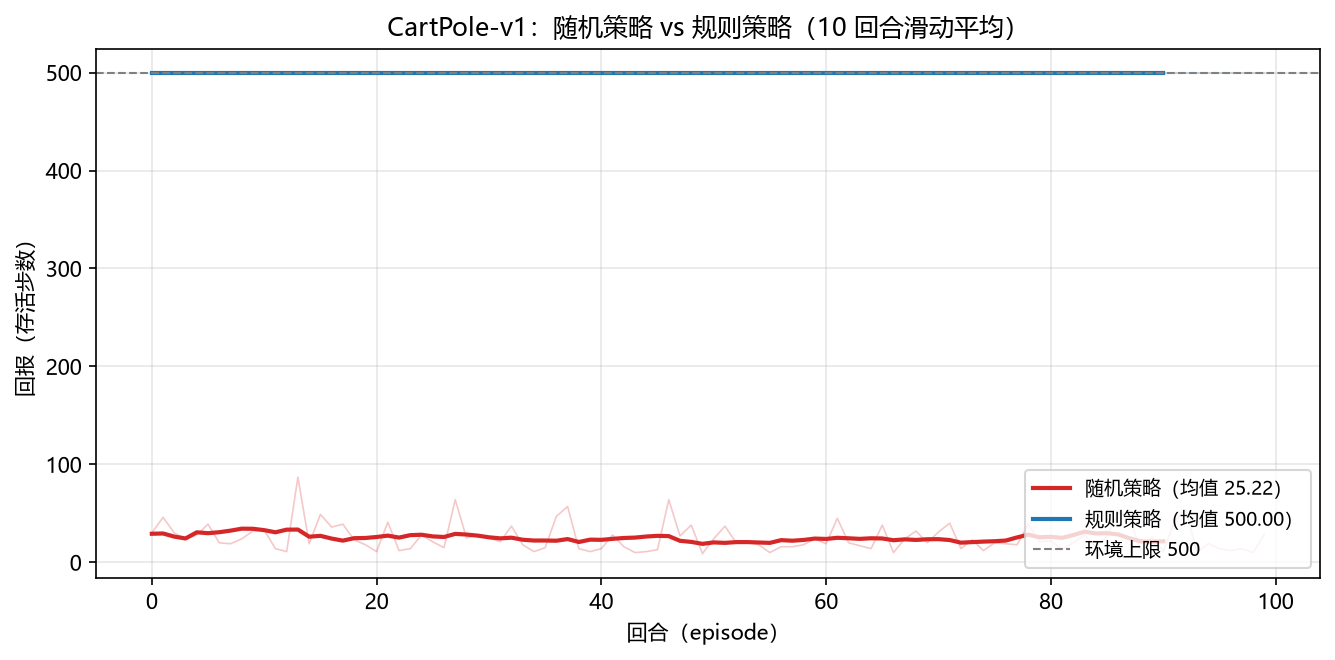
\includegraphics[width=0.92\linewidth]{../figures/L01-return-curves.png}
  \caption{随机策略与规则策略的 100 局回报对比（10 回合滑动平均，seed=42）。浅色为原始值，深色为滑动平均。数据来源：\texttt{experiments/L01-rl-vs-sl/results.csv}。}
  \label{fig:baseline}
\end{figure}

\begin{table}[htbp]
  \centering
  \caption{两种策略的 100 局回报统计（CartPole-v1，seed=42）}
  \label{tab:baseline}
  \begin{tabular}{lcccc}
    \toprule
    策略 & 平均回报 & 标准差 & 最小值 & 最大值 \\
    \midrule
    随机 & 25.22 & 14.12 & 9.00 & 87.00 \\
    规则 & 500.00 & 0.00 & 500.00 & 500.00 \\
    \bottomrule
  \end{tabular}
\end{table}

\section{伪代码：一个完整的交互循环}

\lstinputlisting[style=pseudocode, caption={随机策略的交互循环}, label={alg:loop}]{code/loop.pseudo}

\section{本讲小结}

式~\ref{eq:rl-objective} 是整门课的起点。后面所有的算法——Q-learning、PPO、GRPO——本质上都是在解决
"如何优化这个期望回报"的不同路径。

\begin{keypoint}[下一讲预告]
第 02 讲：MDP 五元组——把决策问题形式化。我们会把"点外卖评分"和"客服对话"各写成一个 MDP。
\end{keypoint}

\end{document}
